%
% File: chap01.tex
% Author: Victor F. Brena-Medina
% Description: Introduction chapter where the biology goes.
%
\let\textcircled=\pgftextcircled
\chapter{Results \& Discussion}
\label{chap:results}

\section{Results}
\paragraph{}

The CLB area and delay were modelled in chapter 2. These models were used to find the optimal LUT size and the CLB was designed. In chapter 2, different switch matrix designs and parameters were explored to find a suitable switch matrix design. The I/O block was designed in Chapter 4. Chapter 5 discussed the programmability of the FPGA. Here, we present the complete schematic of the FPGA designed in Cadence Schematic L:

\begin{figure}[H]
\centering
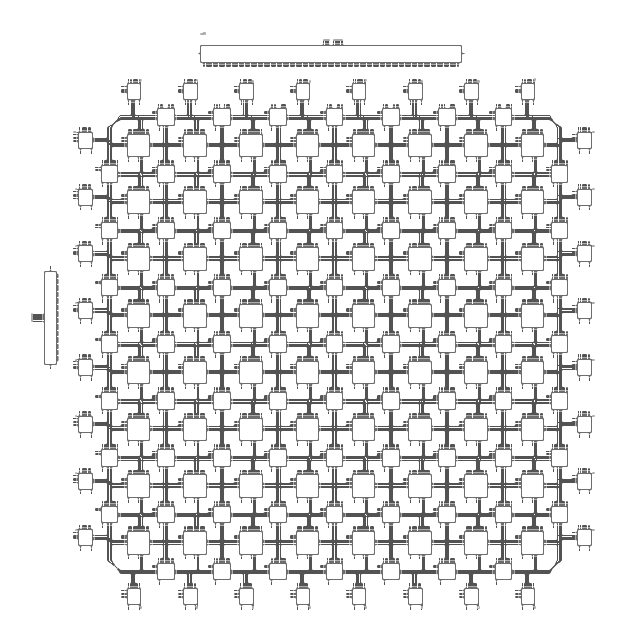
\includegraphics[width=0.9\textwidth]{fpga.png}
\caption{Schematic of the FPGA}
\label{fig:Figure}
\end{figure}

We went on to test the functionality of the FPGA by implementing a 2-bit OR Gate on this FPGA. The bitstream required to program the FPGA was written by hand in an array format as shown below and was parsed using various scripts to automatically generate the relevant stimulus file to program and test the FPGA.

\begin{figure}[H]
\centering
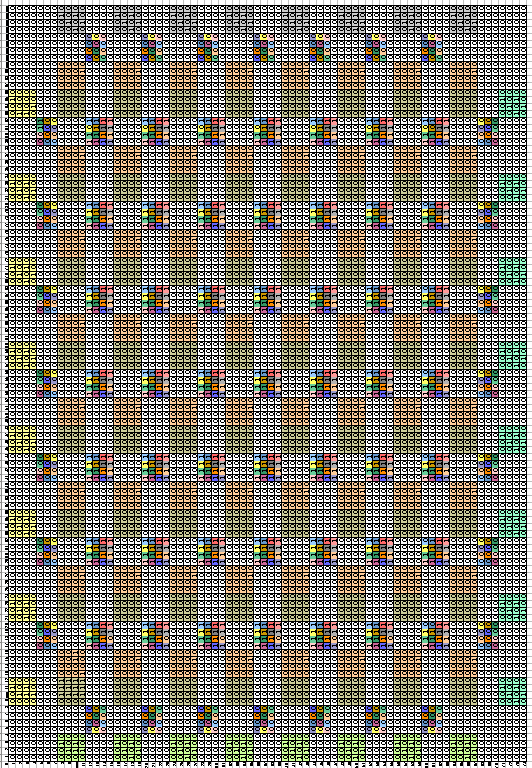
\includegraphics[width=0.9\textwidth]{fpga_bitstream.png}
\caption{Bitstream for 2-input OR gate}
\label{fig:Figure}
\end{figure}

I/O Block left-1 and top-1 are used for inputs and I/O block top-2 is used for output. After programming the FPGA with the bitstream, the waveforms obtained are shown. The delay path for this design is identified as below:

\begin{itemize}
\item \textbf{Output fall time : $36ns$}
\begin{itemize}
\item \textbf{I/O Block top-1 : } The total delay in this block is $7.43ns$ which breaks down as follows:
\begin{itemize}
\item Input buffer : $0.35ns$
\item 2X1 MUX : $0.14ns$
\item 4X1 Crossbar : $6.94ns$
\end{itemize}
\item \textbf{CLB 1 : } The total delay in this block is $24.44ns$ which breaks down as follows:
\begin{itemize}
\item 4X4 Crossbar : $0.19ns$
\item 2X1 MUX : $1.25ns$
\item 2X1 MUX : $2.95ns$
\item 4X1 Crossbar : $20.05ns$
\end{itemize}
\item \textbf{Switch Matrix : } The total delay in this block is $3.94ns$
\item \textbf{I/O Block top-2 : } The total delay in this block is $0.19ns$ which breaks down as follows:
\begin{itemize}
\item 4X1 Crossbar : $0.17ns$
\item Tx-Gate : $0.02ns$
\end{itemize}
\end{itemize}
\item \textbf{Output rise time : $50ns$}
\end{itemize}

The operating frequency for this design comes out to be $\approx$ $20Mhz$ based on schematic level simulations. We might expect a degradation of around 2 after layout and thus say that the design will work at $\approx$ $10Mhz$ for safety.

\begin{figure}[H]
\centering
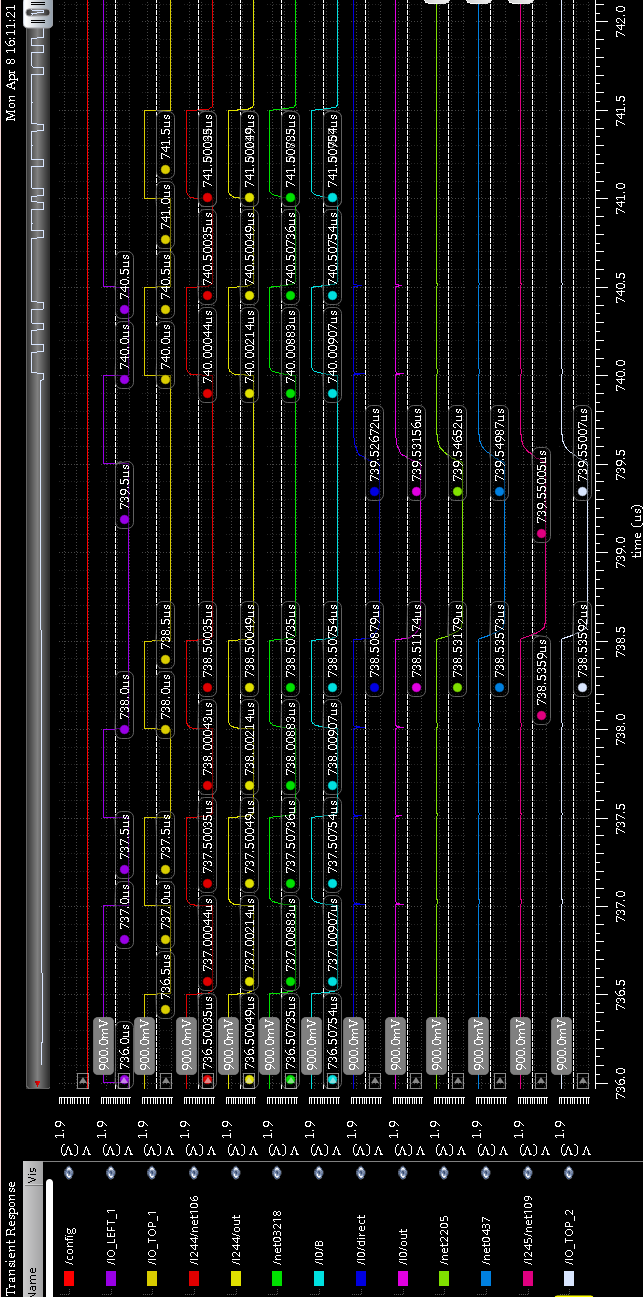
\includegraphics[width=0.77\textwidth]{Short_OR_Delays.png}
\caption{Output waveforms for an OR Gate}
\label{fig:Figure}
\end{figure}

\section{Discussion}
\paragraph{}

We develop models and approximations to help architect an Island-Style FPGA. The models/experiments help to decide critical design parameters like LUT size, routing width etc. The FPGA schematic is then designed from CLB, switch matrix, I/O block and decoder schematics which themselves are made up of smaller schematics. The FPGA functionality is then tested to see the delay path and programming is verified. Although, we have used Cadence Schematic L to proove the design decisions involved, this flow is not suitable for bigger FPGAs. The simulation of a small OR Gate implementation took hours and thus it is not recommended to go beyond that. The designer, after doing a preliminary analysis and testing, can shift to a completely automated digital flow from Verilog to layout. Part of the reason we didn't chose that flow is that SCL $180nm$ PDK is known to have incomplete file structure for a smooth digital flow. Moreover, ours is a small and repetitive design and thus, the layout can even be done by hand. 
